\documentclass{article}
\usepackage[utf8]{inputenc}
\usepackage{listings}
\usepackage{amsmath}
\usepackage{nth}

\title{An empirical study of semantic similarity in WordNet and Word2Vec}
\author{Abe Handler}
\date{\today}
\usepackage{graphicx}
\begin{document}

\begin{abstract}
Google's unsupervised Word2Vec system attempts to determine the semantic distance between words at web scale. This paper performs an empirical analysis of Word2Vec's determinations by comparing them to WordNet, a well-known, human-curated lexical database. It finds that Word2Vec tends to uncover more of certain types of semantic relations than others, with Word2Vec returning more hypernyms than synonyms followed by meronyms, hyponyms and holonyms. Moreover, it shows the likelihood that neighbors separated by distance k in Word2Vec are semantically related in WordNet.
\end{abstract}

\maketitle

\section{Introduction}

Word2Vec is a new unsupervised system for determining the semantic distance between words. For instance, after learning from billions of web pages, Word2Vec reports that the words \textit{Chinese rive} are semantically close to the word \textit{Yangtze}. \cite{Word2VecWebsite} Such results have attracted lots of recent attention: over 100 researchers have cited Word2Vec since its publication in 2013. Yet certain aspects of the system's output are poorly understood. In particular: 

\begin{enumerate}
\item Word2Vec does not label particular semantic relationships between words -- like the synonomy between \textit{cold} and \textit{chilly} or the meronomy between \textit{wheel} and \textit{car}. Instead, it assigns a number between 0 and 1, indicating the semantic distance between two words\footnote{For instance, a Word2Vec model trained on the Google news corpus returns a semantic distance of .390 between \textit{truck} and \textit{tire} and a semantic distance of .168 between \textit{truck} and \textit{chicken}}. However, as Word2Vec’s creators note ``there can be many different types of similarities.” \cite{mikolov2013efficient} This opens a question: what sorts of semantic similarities does Word2Vec uncover?

\item Word2Vec can generate ranked lists showing which words are closer are further way in a semantic model. For example, Word2Vec says that \textit{grandmaster} is \nth{3} from the word \textit{chess}, while \textit{Muay Thai kickboxing} is \nth{997}. \footnote{Word2Vec model trained on Google news corpus} What is the probability that two words that are k-apart in Word2Vec stand in some formal specific semantic relationship?
\end{enumerate}

This study seeks to answer such questions by comparing Word2Vec's output with WordNet -- a large, human-curated ``lexical database" \cite{Wordnetwebsite} and the most-frequently cited ``lexiographic resource" \cite{widdows} in English. 

Such effort has several motivations. First, the study simply gives clearer knowledge of Word2Vec, which is still not well understood. Second, as researchers and practitioners build semantic tools from Word2Vec, they will inevitably turn to WordNet to evaluate their applications. Rei et. all \cite{rei2014looking} have already tried using WordNet to benchmark their Word2Vec-based hyponym detector. Accurately benchmarking such tools requires a clear understanding of the relationship between the two semantic systems. For instance, to evaluate Rei's study, we must ask: what is the probability that Word2Vec will return a holonym from a random word at a semantic distance of k? This study establishes such a baseline for further research. 

\section{Related Work}

\subsection{Word2Vec}
Word2Vec uses complex, multi-level neural networks to determine semantic distance. It's output is a  space filled with vector representations of words. Word vectors that are closer together are more closely related than word vectors that are farther apart. 

The approach has garnered lots of attention and enthusiasm. Researchers have tried using Word2Vec to find the meaning of a word in context \cite{wang2014introduction}, to automatically determine human attitudes in text \cite{xue2014study} and even to ascertain political ideology \cite{iyyerpolitical}. 

Yet no empirical studies have yet attempted to systematically analyze output from Word2Vec in terms of the classical tool, WordNet. 

The gap is notable, in part, because researchers have begun to evaluate such tools using human-curated WordNet -- which remains the most-precise method for determining semantic relationships with a computer.

Rei et. all's ``Looking for Hyponyms in Vector Space" serves as an important example. \cite{rei2014looking} The researchers first use Word2Vec to find words with a particular semantic relationship (hyponomy) -- then look to WordNet to evaluate their method. Yet they presuppose certain relationships between WordNet and Word2Vec without providing any empirical justification, writing that ``the most likely candidates for a high cosine similarity are synonyms, antonyms, hypernyms and homonyms". In section \ref{binary} we show that this is not the case. Word2Vec does not in fact return these semantic relations equally. 

Clearer understanding of how WordNet and Word2Vec are related will yield much precise evaluations. After all, both the linguistic mechanisms and the exact output of the Word2Vec system are still a bit mysterious. One popular explanation of the system concludes: ``Why does this produce good word representations? Good question. We don’t really know." \cite{goldberg2014word2vec}

\subsection{WordNet}  \label{WordNet}
WordNet has been a part of natural language processing for decades -- beginning at Princeton University in 1986. The system has its own logic and jargon, all built around the fundamental building block \cite{wordnet} of the ``synonymous set" (or synset) -- an unordered collection of ``cognitively synonymous words and phrases." \cite{cruse} Synsets are linked by relations, with particular relations linking particular words with particular parts of speech.

Thus, where Word2Vec represents words as vectors, WordNet models language with a large graph -- with semantically similar words (caled ``synsets") serving as the nodes and semantic relationships (such as the meronomy between \textit{tire} and \textit{car}) serving as the edges. 

\footnote{Because ``the majority of the WordNet’s relations connect words from the same part of speech (POS) ... WordNet really consists of four sub-nets, one each for nouns, verbs, adjectives and adverbs, with few cross-POS pointers."\cite{Wordnetwebsite}}

Five specific WordNet relationships concern us here:

\begin{itemize}

  \item \textbf{Synonomy}. WordNet can identify synonyms, words with the same meaning. For instance: \textit{roof} and \textit{ceiling}.
  \item \textbf{Hypernomy}. A word that is more general than some other word is said to be its hypernym. \textit{Language} is a hypernym of \textit{French}
  \item \textbf{Hyponomy}. A word that is more specific than some other word is said to be its hyponym. \textit{French} is a hyponym of \textit{language}
  \item \textbf{Meronomy}. A word that is a part of some other word is called a meronym. \textit{Bedroom} is a meronym of \textit{house}.
  \item \textbf{Holonomy}. If B contains A, B is a holonym of A. \textit{Japan} is a holonym of \textit{Fuji} because Fuji is in Japan.
\end{itemize}

Note that these are relationships between synsets, not between words. A word is associated with one or more synsets. A synset has a semantic relationship with other synsets. We explain our exact definition of semantic relation in the section \ref{method}.

\section{Method} \label{method}
If word vectors represent semantic similarity, we might expect a that two words that are a distance of k apart in Word2Vec have some semantic relationship in WordNet. But what is the probability of this relationship? We investigate with the following experiment. 

We begin with Google's word model, trained on 100 billion words in the Google news corpus \cite{Word2VecWebsite}. Then we randomly select 10,000 words from the Reuters news corpus and, for each, we search for the closet 200 neighbors in the Word2Vec model. We then search WordNet for any semantic relationship between the original word and its neighbor. We only concern ourself with the semantic relations listed in section \ref{WordNet}. 

We allow two words to stand in multiple semantic relationships. For instance, a word is permitted to be both a hyponym and a holonym, if so labeled in WordNet. We also keep track of words that do not appear in WordNet and words that have the same stem -- like \textit{nearing} and \textit{nears}. In these two cases, we do not search for the semantic relationships in WordNet because the relationship is already known. We do not consider antonyms as Wordnet defines anyonyms between words -- not between synsets -- and all other relations are defined between synsets. 

We access WordNet 3.0 and the Reuters-21578 \cite{rose2002reuters} corpus with the Python linguistics toolkit, NLTK \cite{BirdKleinLoper09}. We access the Google news model via the popular python wrapper, Gensim \cite{gensim}. We use NLTK's snowball stemming tool to find words with the same stem. 

We use a binary measure to determine semantic relatedness in WordNet: if there is any overlap between the relevant synsets, we count the relation. If there is zero overlap between the synsets, we do not count the relation. For instance, our experiment might determine that \textit{introduction} and \textit{initiation} are synonyms because their synsets overlap with the synset 'initiation.n.01' -- defined as 'a formal entry into an organization or position or office'. 

Finally, some relations in WordNet have more associated synsets than others. Thus our experiment might be said to measure differences in associated synsets in WordNet instead of output from Word2Vec. We address this deficiency by generating adjusted counts that show the probability of each relation -- if all relations contained equally many synsets. We do this as follows. First we randomly sample 10,000 words from the Reuters corpus and determine the average number of associated synonyms, meronyms, holoynms, hypernyms and hyponyms. Then we average these averages to get an overall average number of associated synsets. To generate an adjusted count for some relation, we multiply the raw count by the overall average divided by the average for synset. Thus, if some synset has twice as many associated words than average its count will be halved. If some synset has half as many as the overall average, its output will be doubled.

\section{Results}

\subsection{What kinds of relations does Word2Vec return?} \label{binary}
In general, Word2Vec finds more synonyms, hyponyms and hypernyms than meronyms and holonyms. The overall pattern is shown in Fig. \ref{fig:all} on page \pageref{fig:all}.
\begin{center}
\centering
    \begin{tabular}{ | l | l | l | l | l | l |}
    \hline
Relation & k less than 40 & k=40-80 & k=80-120 & k=120-160 & k=160-200 \\  \hline
Synonomy &5120 & 1671 & 1085 & 814 & 617\\  \hline
Hyponomy &2874 & 1261 & 865 & 781 & 589\\  \hline
Hypernomy &4593 & 2149 & 1564 & 1160 & 1004\\  \hline
Holonomy &161 & 63 & 47 & 35 & 26\\  \hline
Meronomy &339 & 112 & 69 & 60 & 55\\  \hline
Same stem &13333 & 1820 & 1145 & 782 & 608\\  \hline
Not in wordnet &90092 & 90074 & 90063 & 90060 & 90052\\  \hline
Key Error* &  All k = 1764 \\  \hline
    \end{tabular}
\end{center}
*Key Errors occur when a word from the Reuters Corpus does not occur in the Word2Vec model. Many come from when NLTK considers a number or punctuation mark a word.

\begin{figure}[!hb]
  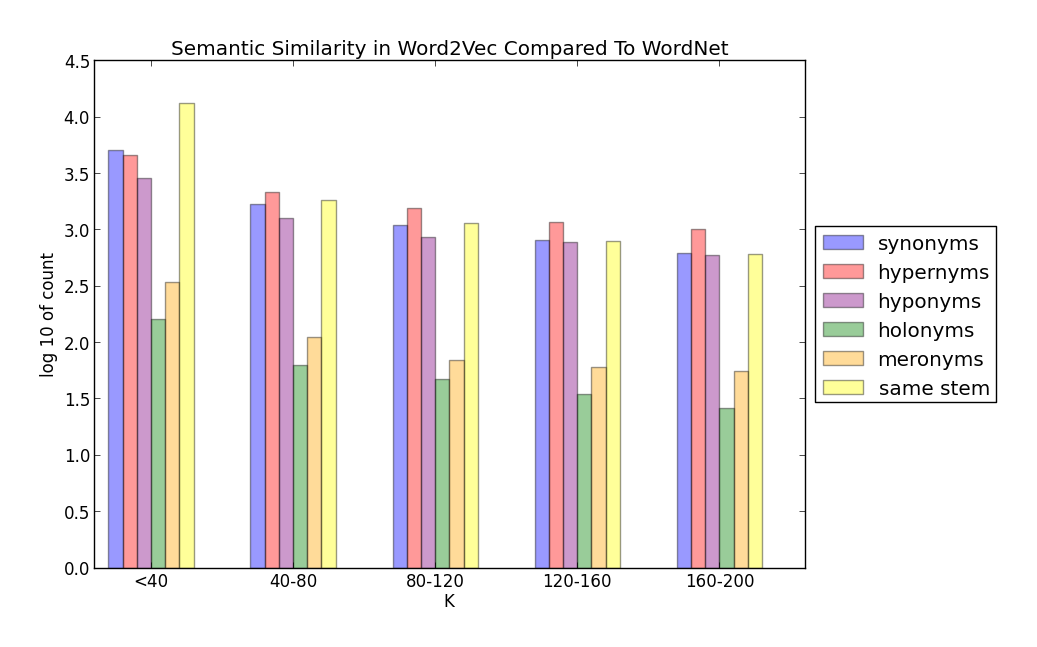
\includegraphics[scale=.5]{All.png}
  \caption{Word2Vec finds more hypernyms and synonyms than meronyms, hyponyms and holonyms. It finds fewer of all of the kinds of relations as k increases, meaning that words are less likely to be related in WordNet as their semantic distances grow farther away.}
  \label{fig:all}
\end{figure}

We find that by far the largest category are those results that do not appear at all in WordNet. This is because the model trained on the Google news corpus with Word2Vec is much, much larger than all of WordNet. Where WordNet 3 contains around 118,000 synsets \cite{wordnet}. The Word2Vec model in this experiments was trained on 100 billion words \cite{Word2VecWebsite} of news text. Most of the semantically similar words cannot be looked up in WordNet. For instance, \textit{Rohto Pharmaceutical} is not in WordNet: it's a big corporation, but not a household name in the United States. Thus WordNet has no way of determining its semantic relationship to the word \textit{industries}.\footnote{The Google news Word2Vec model lists the semantic distance between \textit{Rohto Pharmaceutical} and \textit{industries} at .494} It is not known how well the WordNet relations represent the mass of `semantically similar' words in Word2Vec. We consider this in section \ref{Future Work}.

\subsection{Values of K} \label{val_k}
There are far fewer WordNet relations across all categories as k gets larger.  In other words, the greater the semantic distance (in Word2Vec), the greater the value of k and the less likely that two words are semantically related in WordNet. This is as expected, provided that Word2Vec's determinations of semantic distance are reliable.

\begin{figure}[!hb]
  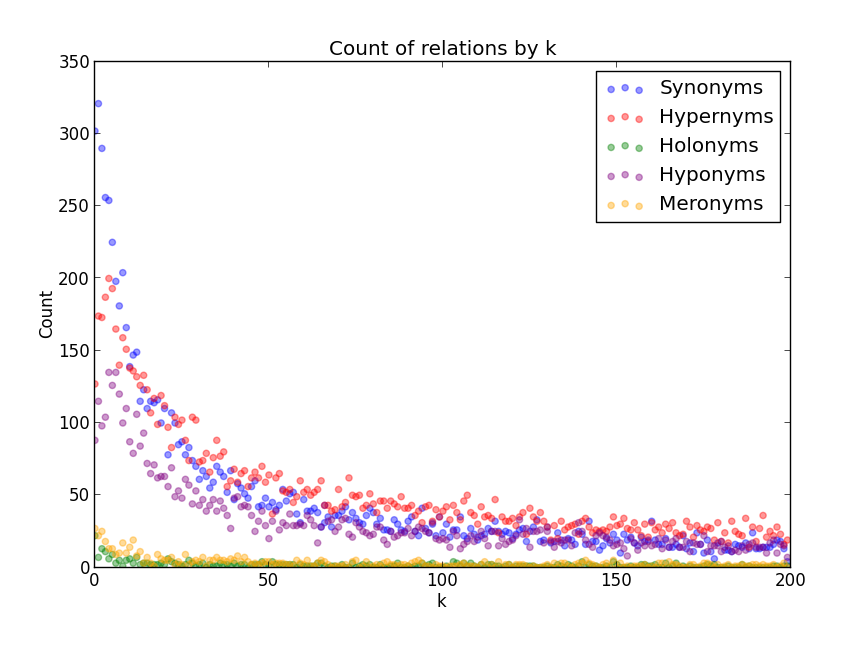
\includegraphics[scale=.5]{total.png}
  \caption{For all types of relations, the number of relations drops as k increases. As words are further apart in Word2Vec they are less likely to be related in WordNet. Counts of meronyms and holonyms drop off towards zero once k gets much greater than ten.}
  \label{fig:all_counts}
\end{figure}

That said, there are certain key differences between hypernyms, hyponyms and synonyms as compared with meronyms and holonyms. As k increases, counts of meronyms and holonyms drop to almost zero. But counts of hypernyms, hyponyms and synonyms level off to a constant rate, higher than zero. It would be interesting to determine at what point such relations also become, in essence, zero. We discuss this in section \ref{Future Work}.

\subsection{Probabilities}
Researchers who try to find particular kinds of relations using Word2Vec need to understand the baseline probability of the the relation at a particular semantic distance. Effective tools should beat such a probability. An effective holonym detector, for instance, should beat the average probability of a holonym at a given semantic distance. 

Our experiment uncovered such probabilities, which we present here. We exclude meronyms and holonyms from this analysis because, as k increases past approximately 10, their probability becomes very very close to zero, as discussed in section \ref{val_k}.

\begin{figure}[!hb]
  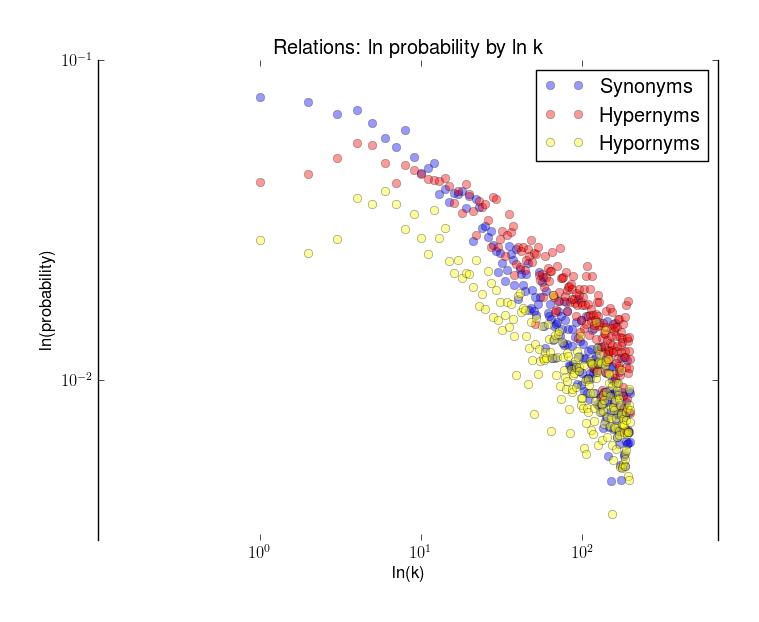
\includegraphics[scale=.7]{loglog_prob.png}
  \caption{Word2Vec is more likely to find synonyms at low values of k. But as k increases, it is more likely to find more hypernyms.}
  \label{fig:loglog_prob}
\end{figure}

\subsection{Adjusted counts}
To what extent do differences in the relative synset sizes explain the different sorts of relations uncovered by Word2Vec? For instance, if words have more synonyms than holonyms, then it would make sense for Word2Vec to find more synonyms than holonyms. Thus, we revisit the results from section \ref{binary} with adjusted counts.

To find an adjusted count, we take the average number of each type of relation returned for a particular word. We find the max of each of those numbers. And, for each relation that is not the maximum, we find that number as a fraction of the maximum. The adjusted count is 1 over the inverse of that number times the actual count. So if the average synset size for meronyms is 1/4 smaller than the average synset size of hyponyms (the biggest), the meronym count would increase by 1/.25 = 4.

\begin{figure}[!ht]
  \begin{minipage}{0.7\textwidth}
    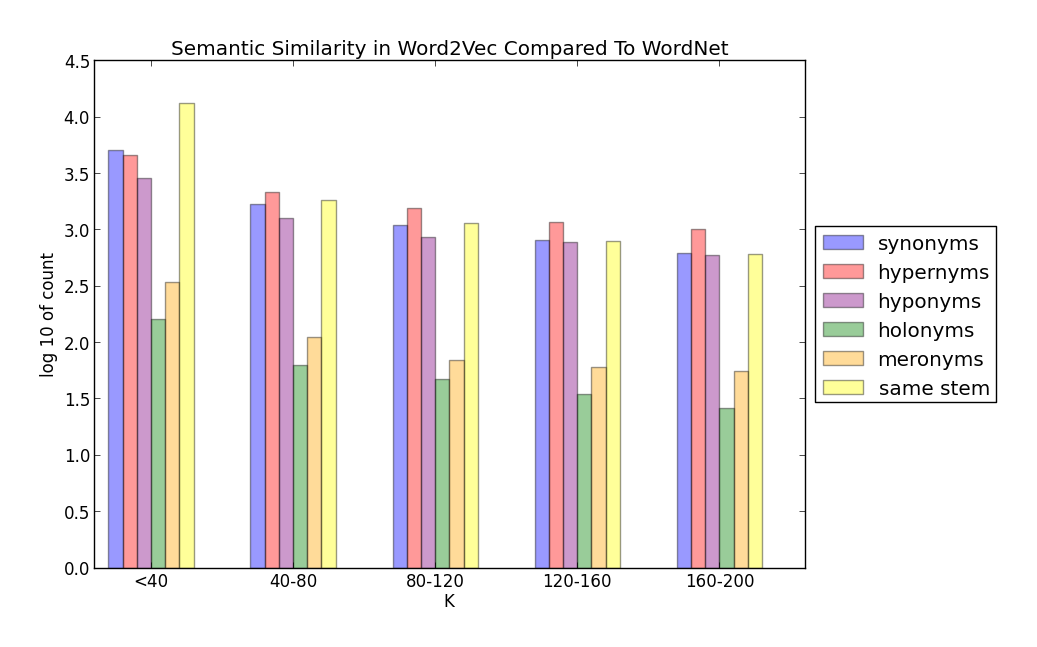
\includegraphics[width=\textwidth]{All.png}
    \caption{Counts from section \ref{binary}}
  \end{minipage}
 
  \begin{minipage}{0.7\textwidth}
    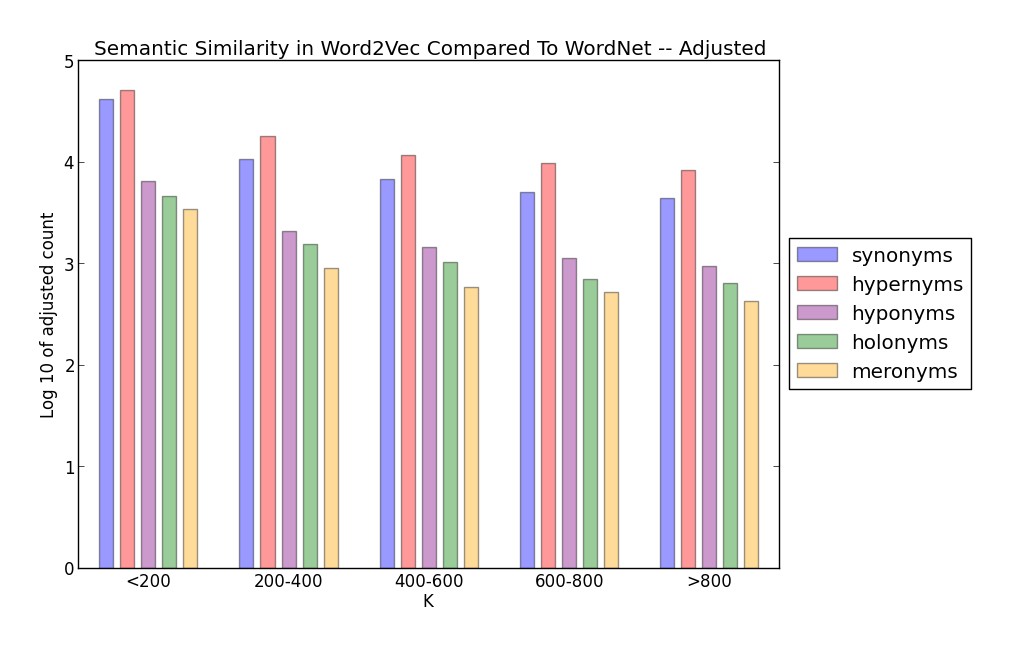
\includegraphics[width=\textwidth]{Adjusted.png}
    \caption{Counts adjusted for synset size}
  \end{minipage}
\end{figure}

Adjusted counts give a different perspective on Word2Vec. They show that, in general, Word2Vec returns more hypernyms than synonyms -- followed by hypernyms, holonyms and meronyms. 

\section{Future Work} \label{Future Work}

Comparing WordNet and Word2Vec is a limited topic and it has been thoroughly covered here. Most future work on Word2Vec will involve building tools and algorithms using word vectors. This study provides a clear baseline for such efforts. We hope that others use it to benchmark tools. 

That said a few matters of comparison have been left uncovered. 

In section \ref{val_k} we show that as k increases, Word2Vec eventually stops finding meronyms and holonyms (with any regularity). But it continues to find synonyms, hypernyms and hyponyms as k extends past 200. At what value of k does Word2Vec stop finding relations? This is not answered in this study.

Additionally, this study uses one measure of semantic distance, k -- which is explained in section \ref{method}.
However, Word2Vec projects word vectors into semantic space. Thus, the system allows for any number of different measures of geometric distance, like Euclidean distance or Manhattan distance. Such geometric distances might yield different results. The might need to be investigated, depending on the particular needs at hand. 

Finally, this study only considered the text of news articles. It would be interesting to compare Word2Vec's performance on different sorts of text. Do news articles tend to favor words at higher levels of generality (hypernyms) over words at lower level of generality (hyponyms)? If so, experimenters might find different results. 

\appendix
\section{Jacard index}
In our experiment, we use a binary measure of relatedness: if relevant synsets overlap, we consider the words related. Again, our experiment would determine that \textit{introduction} and \textit{initiation} are synonyms because their synsets overlap with the synset 'initiation.n.01'.  This opens a potential complicating problem: the simple binary determination does not take into account that the word ``introduction" has seven associated synsets but the word ``initiation" has only 4 synsets -- and that these two sets overlap on a single synset. To account for the relative degree of overlap, we also take the Jaccard index of the overlapping sets to gain a better sense of the degree to which semantically related words are related.

Results in section \ref{binary} consider any overlap between synsets as a  ``relation". For instance, consider a given word pair A,B. Imgine that Wordnet gives 3 synsets as hyponyms of A and gives 5 synsets for B. If one of the synsets that are hyponyms of A matches one of the 5 synsets for B then we consider this a hyponym. However, are certain types of relation closer than others? We investigate this by examining the Jaccard coefficient of each linked relation -- i.e. the intersection of two sets divided by their union. Our findings are shown in figure \ref{fig:jacard}.

\begin{figure}[!ht]
\centerline{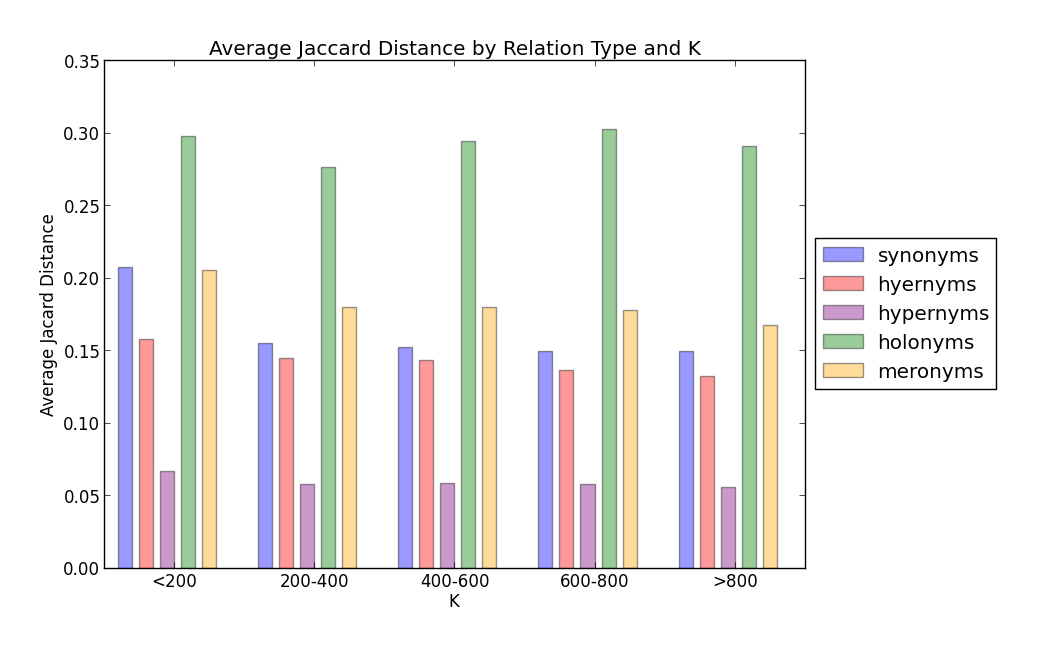
\includegraphics[scale=.5]{jacard.png}}
  \caption{Jaccard indexes vary depending on type of relation -- but the variation is closely correlated to the different sizes of synsets in WordNet}
  \label{fig:jacard}
\end{figure}

At first glance, figure \ref{fig:jacard} seems to show that Jacard indexes vary. However, we sampling 10,000 words from the Reuters corpus and finding the average number of synonyms, hypoynms, hypernyms, holonyms and meronyms associated with each word (excluding zeros) shows that Jaccard indexes for a given type of relation are strongly linked with the average synset sizes for each type of relation in WordNet.

\begin{center}
\centering
    \begin{tabular}{ | l | l |}
    \hline
Relation & Relative sizes of types of synsets in Wordnet \\  \hline
Synonomy & .141 \\  \hline
Hyponomy & .576  \\  \hline
Hypernomy & .132 \\  \hline
Holonomy & .049 \\  \hline
Meronomy & .100 \\  \hline
    \end{tabular}
\end{center}

In other words, the Jaccard index for holonyms is highest -- but the holonymm set has the lowest average size in WordNet. This means that for holonyms, the denominator in the index will be smaller and the overall value will be greater. Similarly, the Jaccard index for hyponyms is lower because the average number of hyponyms is greater. Differences in Jaccard indexes seem largely attributable to differences in synset sizes in WordNet (or perhaps in English), not to differences in the semantic relations uncovered by Word2Vec.


\bibliographystyle{unsrt}%Used BibTeX style is unsrt
\bibliography{sample}

\end{document}
